\pdfoutput=1
\documentclass[11pt,a4paper]{article}
\usepackage{abhijit-research}
\renewcommand{\PaperCode}{P14}
\renewcommand{\PaperKind}{RESEARCH PAPER}
\renewcommand{\PaperVersion}{VERSION 1.0}
\renewcommand{\PaperDate}{AUGUST 2026}
\renewcommand{\PaperTitle}{Past-Unbounded Cosmology}
\renewcommand{\PaperSubtitle}{An Exact Dust-Vacuum Return Condition}
\renewcommand{\PaperFullTitle}{Past-Unbounded Cosmology and an Exact Dust-Vacuum Return Condition}
\renewcommand{\PaperShortTitle}{Past-Unbounded Cosmology}
\renewcommand{\PaperKeywords}{cosmology; dark energy; cosmic age; acceleration; recurrence; horizons}
\renewcommand{\PaperClassification}{The numerical values are exact conditional consequences of the displayed model and returned-present postulate. They are not an observational fit. Absolute scale, perturbations, and a full likelihood remain open.}
\renewcommand{\PaperCitation}{Singh, Abhijit. 2026. \textit{Past-Unbounded Cosmology and an Exact Dust-Vacuum Return Condition}. Research manuscript, version 1.0.}
\begin{document}
\MakeResearchTitle
\MakeResearchContents
\MakeResearchAbstract{%
A past-unbounded causal history is separated from the finite age of a particular cosmological branch. In a flat dust-plus-vacuum model, acceleration onset and matter-vacuum equality are distinct. Applying a declared complement return to the acceleration boundary gives an exact present vacuum fraction of two thirds. Without fitting within the branch, this condition forces $z_{\rm acc}=0.587401052$, $z_{\rm eq}=0.259921050$, $H_0t_0=0.9358813101$, $\Delta N=0.4620981204$, $q_0=-1/2$, and $j_0=1$. A nonsingular recurrent solution demonstrates mathematical consistency of a past-unbounded class. The paper also proves the absolute-scale obstruction, separates cold-matter and slow-roll requirements, and states a full-path falsification protocol. Black-hole discussion is confined to accessibility and known thermodynamic targets.
}
\section{Past-unbounded histories and typed age}
A causal history is past-unbounded when
\begin{equation}
\forall e\;\exists e'\quad e'\prec e.
\end{equation}
This condition is compatible with finite ages for particular thermodynamic or geometric phases. A total age function cannot be both invariant under arbitrary origin shift and increase by one under every update. A past-unbounded model therefore has no unique origin-independent total age, while phase ages remain well defined relative to physical transitions.

\section{Flat dust-vacuum branch}
Consider a spatially flat Friedmann model with pressureless matter and a constant vacuum term:
\begin{equation}
H(a)^2=H_0^2\left(\Omega_{m,0}a^{-3}+\Omega_{\Lambda,0}\right),
\qquad \Omega_{m,0}+\Omega_{\Lambda,0}=1.
\end{equation}
Let $p=\rho_\Lambda/(\rho_m+\rho_\Lambda)$. In e-fold time $N=\log a$,
\begin{equation}
p'=3p(1-p).
\end{equation}
Acceleration begins at $p=1/3$. The declared complement return maps this boundary to
\begin{equation}
\boxed{p_{\rm ret}=2/3.}
\end{equation}
Identifying the present epoch with the returned event is the model's physical postulate. The consequences below are exact after that postulate.

\section{Exact dimensionless predictions}
Matter-vacuum equality satisfies $\rho_m=\rho_\Lambda$, while acceleration onset satisfies $\rho_m=2\rho_\Lambda$. With $(\Omega_{m,0},\Omega_{\Lambda,0})=(1/3,2/3)$,
\begin{align}
z_{\rm eq}&=2^{1/3}-1=0.259921050,\\
z_{\rm acc}&=2^{2/3}-1=0.587401052.
\end{align}
The age integral is
\begin{equation}
H_0t_0=\int_0^1\frac{da}{a\sqrt{\Omega_{m,0}a^{-3}+\Omega_{\Lambda,0}}}
=\frac{2}{3\sqrt{\Omega_{\Lambda,0}}}
\operatorname{arsinh}\sqrt{\frac{\Omega_{\Lambda,0}}{\Omega_{m,0}}}.
\end{equation}
Therefore
\begin{equation}
\boxed{H_0t_0=\sqrt{\frac23}\operatorname{arsinh}\sqrt2=0.9358813101.}
\end{equation}
The logarithmic expansion interval associated with the returned fraction is
\begin{equation}
\boxed{\Delta N=\frac23\ln2=0.4620981204.}
\end{equation}
The present deceleration and jerk are
\begin{equation}
q_0=\frac12\Omega_{m,0}-\Omega_{\Lambda,0}=-\frac12,
\qquad j_0=1.
\end{equation}
The fraction of branch age elapsed since acceleration began is $0.4255192360$.

\begin{figure}[H]\centering
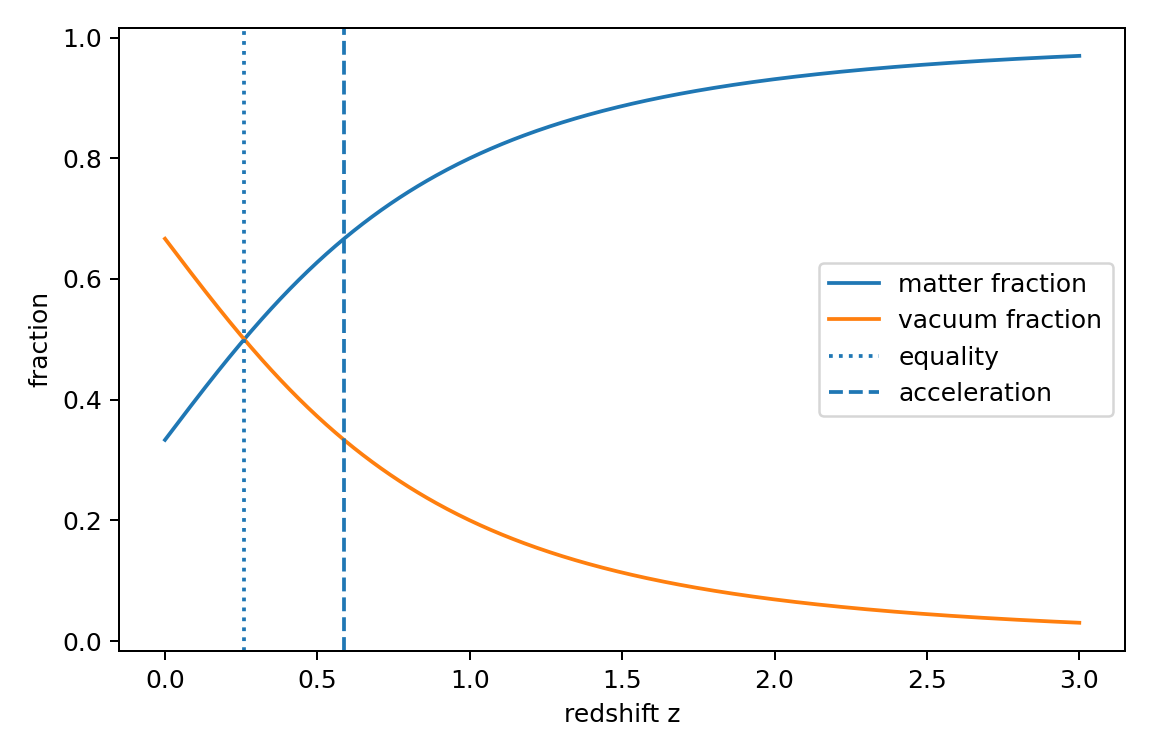
\includegraphics[width=.72\linewidth]{figures/p14_density_fractions.png}
\caption{Exact matter and vacuum fractions in the returned dust-vacuum branch.}
\end{figure}

\begin{figure}[H]\centering
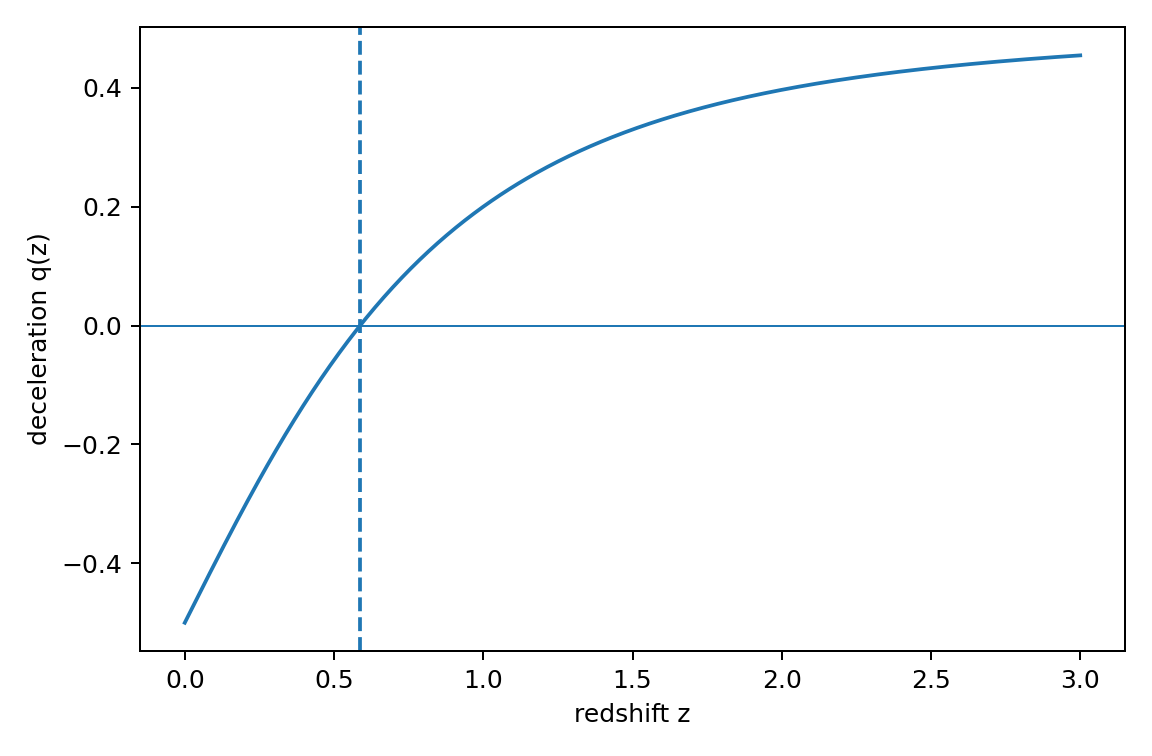
\includegraphics[width=.72\linewidth]{figures/p14_deceleration.png}
\caption{Deceleration parameter; the zero crossing is the exact acceleration redshift.}
\end{figure}

\section{Comparison with one external parameter estimate}
Using the Planck 2018 flat-$\Lambda$CDM estimate $\Omega_{\Lambda,0}\simeq0.6847\pm0.0073$, the value $2/3$ differs by approximately $2.47$ quoted standard deviations. This comparison is model dependent and not a full likelihood analysis. It makes the returned-present postulate sharp and already constrained rather than adjustable.

\section{Scale obstruction}
All results above are dimensionless. The dilation
\begin{equation}
H\mapsto\mu H,\qquad t\mapsto t/\mu
\end{equation}
leaves the dimensionless history invariant. No absolute $H_0$, age in years, vacuum energy density, sound horizon, or physical parent scale follows without one additional dimensionful input generated by the model.

A later controlled transmutation map gives an exact conditional relation between a symmetry scale, coupling data, and an absolute age. The physical vacuum formation and its parameters are not yet derived, so the map is retained as a conditional calibration route rather than a numerical prediction.

\section{Past-unbounded recurrent example}
The equation
\begin{equation}
\ddot\chi+\omega^2(\chi-\chi_*)=0
\end{equation}
has $\chi=\chi_*+A\cos(\omega t+\phi)$. Setting $J_g=e^\chi$ gives a positive scale factor
\begin{equation}
a(t)=\exp\left[\frac{\chi_*+A\cos(\omega t+\phi)}{d_s}\right],
\end{equation}
with alternating expansion and contraction. This proves mathematical consistency of a nonsingular past-unbounded class; it does not identify the observed universe.

\section{Dark sectors}
A cold dark-matter component must have negligible pressure, cluster gravitationally, and approximately scale as $a^{-3}$. A coherently oscillating massive scalar can reproduce this background and clustering only when its mass is large relative to the Hubble scale on the relevant epochs.

A late dark-energy component with $w\simeq-1$ requires kinetic energy much smaller than potential energy and an effective mass of order $H_0$ or below if rolling today. One homogeneous quadratic mode cannot simultaneously satisfy both present-day cold-matter clustering and slow-roll dark energy. A unified origin would require distinct modes, phases, condensates, or a constant vacuum term plus an oscillating component.

\section{Horizons and black holes}
An event horizon is a boundary of future accessibility,
\begin{equation}
\mathcal H=\partial J^-(\mathcal I^+).
\end{equation}
Exterior inaccessibility is not identical to global information destruction. A complete microscopic theory must recover
\begin{equation}
S_{\rm BH}=\frac{k_BA}{4\ell_P^2},
\end{equation}
Hawking dynamics, interior continuation, and unitary accounting. The present framework supplies an accessibility interpretation and a two-exponent distinction between residual instability and inaccessible provenance; it does not derive black-hole microstates or evaporation.

\section{Full-path falsification}
The branch must be tested without retuning the returned fraction. The linked functions
\begin{equation}
H(z),\quad q(z),\quad D_A(z),\quad D_L(z),\quad t(z),\quad f\sigma_8(z)
\end{equation}
should be evaluated against a frozen external likelihood. Failure of any linked observable rejects the branch as a physical account while leaving the conditional algebra intact.

\section{Status}
The $2/3$ return and all displayed dimensionless numbers are exact inside the flat dust-vacuum and present-equals-return assumptions. The present-equals-return postulate, absolute scale, perturbation spectrum, sound horizon, and full likelihood remain empirical or open.


\section{Typed age and the absence of a universal origin}
A causal history is past-unbounded when every event has an earlier event. Such a history can contain finite-duration phases without a first event. An origin-independent total age $A$ cannot both satisfy translation invariance $A(n+k)=A(n)$ for arbitrary origin shifts and increment law $A(n+1)=A(n)+1$. Hence a past-unbounded model has no unique total age while a hot, smooth, or observational branch can have a finite age measured from a physical transition.

\section{Exact FLRW derivation}
For flat dust plus a constant vacuum component,
\begin{equation}
E(a)^2=\frac{H(a)^2}{H_0^2}=\Omega_{m,0}a^{-3}+\Omega_{\Lambda,0},
\qquad \Omega_{m,0}+\Omega_{\Lambda,0}=1.
\end{equation}
Under the returned-state condition
\begin{equation}
\Omega_{\Lambda,0}=\frac23,\qquad \Omega_{m,0}=\frac13,
\end{equation}
the matter-vacuum equality condition gives
\begin{equation}
1+z_{\rm eq}=2^{1/3},
\end{equation}
and the acceleration condition $\rho_m=2\rho_\Lambda$ gives
\begin{equation}
1+z_{\rm acc}=2^{2/3}.
\end{equation}
The age integral is
\begin{equation}
H_0t_0=\int_0^1\frac{da}{aE(a)}
=\frac{2}{3\sqrt{\Omega_{\Lambda,0}}}
\operatorname{arsinh}\sqrt{\frac{\Omega_{\Lambda,0}}{\Omega_{m,0}}},
\end{equation}
so
\begin{equation}
H_0t_0=\sqrt{\frac23}\operatorname{arsinh}\sqrt2=0.9358813101.
\end{equation}
The exact branch register is
\begin{center}
\begin{tabular}{lc}
\toprule
quantity&value\\\midrule
$\Omega_{\Lambda,0}$&$2/3$\\
$z_{\rm acc}$&$0.587401052$\\
$z_{\rm eq}$&$0.259921050$\\
$H_0t_0$&$0.9358813101$\\
$q_0$&$-1/2$\\
$j_0$&$1$\\
$\Delta N$&$(2/3)\ln2=0.4620981204$\\
\bottomrule
\end{tabular}
\end{center}
These are forced by the branch assumptions rather than fitted independently.

\section{Past-unbounded recurrent construction}
The equation
\begin{equation}
\ddot\chi+\omega^2(\chi-\chi_*)=0
\end{equation}
has $\chi=\chi_*+A\cos(\omega t+\phi)$. Setting $J_g=e^\chi$ and $a=J_g^{1/d_s}$ gives a positive nonsingular scale factor for all $t$, with alternating expansion and contraction. This proves consistency of one past-unbounded cosmological class; it does not identify the observed universe with that class.

\section{Finite-capacity fate theorem}
If accessible geometric capacity is finite but $H(t)\ge h>0$ for all sufficiently late time, then
\begin{equation}
J_g(t)\ge J_g(t_0)e^{d_sh(t-t_0)},
\end{equation}
which eventually exceeds every finite bound. Thus finite capacity requires $H\to0$, a later sign change, or continuing access to new capacity.

\section{Dark sectors and horizon scope}
A cold dark-matter candidate must cluster and approximately scale as $a^{-3}$; the framework supplies a possible structural role for stable neutral recurrent excitations but no mass, abundance, or cross section. A vacuum component has $p=-\rho$; the two-thirds branch fixes a dimensionless present fraction but does not derive the observed microscopic vacuum scale.

An event horizon is a boundary of future accessibility. Exterior inaccessibility is not identical to global destruction of information. A microscopic theory must recover the area law, its coefficient, Hawking flux, and unitary accounting. The present causal description identifies the boundary problem but does not derive those microphysics.

\section{Full observational test}
Freeze the $2/3$ postulate before comparison. Evaluate the linked functions $H(z)$, $q(z)$, distance measures, age, and growth under a current external likelihood without retuning the return condition. Model comparison must include covariance, priors, and alternatives. A failure of any linked observable rejects the physical branch while leaving the conditional derivation intact.

\begin{thebibliography}{99}
\bibitem{weinberg} S. Weinberg, Cosmology, Oxford University Press, 2008.
\bibitem{planck} Planck Collaboration, Planck 2018 results VI: cosmological parameters, Astronomy and Astrophysics 641 (2020), A6.
\bibitem{malament} D. Malament, The class of continuous timelike curves determines the topology of spacetime, Journal of Mathematical Physics 18 (1977), 1399--1404.
\bibitem{bekenstein} J. D. Bekenstein, Black holes and entropy, Physical Review D 7 (1973), 2333--2346.
\bibitem{hawking} S. W. Hawking, Particle creation by black holes, Communications in Mathematical Physics 43 (1975), 199--220.
\end{thebibliography}
\end{document}
